% ==================================================
% VAE-based Drawing System 
% Author: Lester James V. Miranda
% ==================================================

\documentclass[preview, convert={outfile=\jobname-out.png,density=300}]{standalone}

\usepackage{tikz}
\usepackage{color}
\usepackage{subfig}
\usepackage{ifthen}
\usepackage{graphicx}
\usepackage{fontawesome}

\renewcommand\familydefault{\sfdefault}

\usetikzlibrary{
    matrix,
    shapes,
    fit,
    arrows,
    positioning,
    calc,
    backgrounds,
    shadows.blur,
    shapes.geometric,
}


% taken from manual
\makeatletter
\pgfdeclareshape{document}{
\inheritsavedanchors[from=rectangle] % this is nearly a rectangle
\inheritanchorborder[from=rectangle]
\inheritanchor[from=rectangle]{center}
\inheritanchor[from=rectangle]{north}
\inheritanchor[from=rectangle]{south}
\inheritanchor[from=rectangle]{west}
\inheritanchor[from=rectangle]{east}
% ... and possibly more
\backgroundpath{% this is new
% store lower right in xa/ya and upper right in xb/yb
\southwest \pgf@xa=\pgf@x \pgf@ya=\pgf@y
\northeast \pgf@xb=\pgf@x \pgf@yb=\pgf@y
% compute corner of ‘‘flipped page’’
\pgf@xc=\pgf@xb \advance\pgf@xc by-10pt % this should be a parameter
\pgf@yc=\pgf@yb \advance\pgf@yc by-10pt
% construct main path
\pgfpathmoveto{\pgfpoint{\pgf@xa}{\pgf@ya}}
\pgfpathlineto{\pgfpoint{\pgf@xa}{\pgf@yb}}
\pgfpathlineto{\pgfpoint{\pgf@xc}{\pgf@yb}}
\pgfpathlineto{\pgfpoint{\pgf@xb}{\pgf@yc}}
\pgfpathlineto{\pgfpoint{\pgf@xb}{\pgf@ya}}
\pgfpathclose
% add little corner
\pgfpathmoveto{\pgfpoint{\pgf@xc}{\pgf@yb}}
\pgfpathlineto{\pgfpoint{\pgf@xc}{\pgf@yc}}
\pgfpathlineto{\pgfpoint{\pgf@xb}{\pgf@yc}}
\pgfpathlineto{\pgfpoint{\pgf@xc}{\pgf@yc}}
}
}
\makeatother


\begin{document}
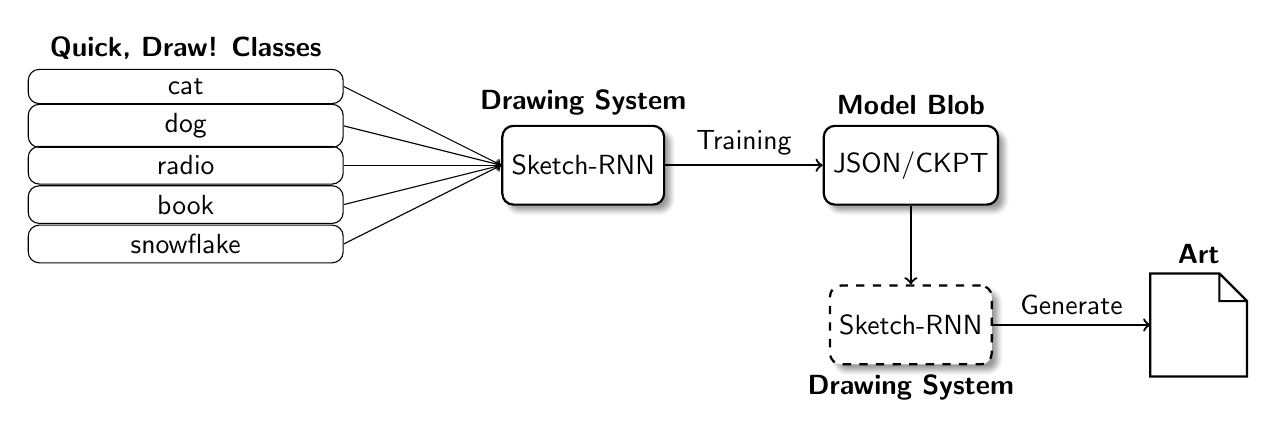
\begin{tikzpicture}[
    node distance= 2cm,
    module/.style={draw, thick, rounded corners, text=black, align=center,
                minimum width=2cm,minimum height=1cm,fill=white, 
                blur shadow={shadow blur steps=5}},
    qd/.style={draw, rounded corners, align=center, minimum width=4cm},
    file/.style={draw, shape=document, minimum width=1.2cm, minimum
                height=1.28cm, thick, fill=white}
]

% QD Classes 
\node[qd, label={\bfseries Quick, Draw! Classes}] at (0,0) (class0) {cat};
\node[qd] at (0,-0.5) (class1) {dog};
\node[qd] at (0,-1.0) (class2) {radio};
\node[qd] at (0,-1.5) (class3) {book};
\node[qd] at (0,-2.0) (class4) {snowflake};

% Drawing System1 
\node[module, label={\bfseries Drawing System}] [right=of class2]
    (DrawingSystem) {Sketch-RNN};

\draw[->] (class0.east) -- (DrawingSystem.west) {};
\draw[->] (class1.east) -- (DrawingSystem.west) {};
\draw[->] (class2.east) -- (DrawingSystem.west) {};
\draw[->] (class3.east) -- (DrawingSystem.west) {};
\draw[->] (class4.east) -- (DrawingSystem.west) {};

% Model Blob
\node[module, label={\bfseries Model Blob}] [right=of DrawingSystem]
    (Blob) {JSON/CKPT};

\draw[->, thick] (DrawingSystem) -- (Blob) node[pos=0.5, above] {Training};

% Drawing System2 
\node[module,dashed,  label=below:{\bfseries Drawing System}] [below=of Blob,
    yshift=1cm] (DrawingSystem2) {Sketch-RNN};

\draw[->, thick] (Blob) -- (DrawingSystem2) {};

% Output image
\node[file, label={\bfseries Art}] (OutputImage) [right=of DrawingSystem2] {};

\draw[->, thick] (DrawingSystem2) -- (OutputImage) node[pos=0.5, above] {Generate};

\end{tikzpicture}
\end{document}

